The following problems are designed to familiarize you with concepts you will use throughout the lab. We will tackle four topics topics:
\begin{enumerate}
	\item Performing compression using the SVD on image data
	\item Working with video data in MATLAB
	\item Performing compression using the SVD on frames of video data
	\item Reshaping video data to achieve the main results of the lab
\end{enumerate}

\subsection{Compressing image data}
From class, you will remember the Eckart-Young Theorem
\begin{theorem}
	Given a matrix, $A \in \set{R}^{m \times n}$ that has rank $r$, we can find a rank $k \leq r$ approximation to $A$, $X$ as
	$$\sum_{i = 1}^k \sigma_i u_i v_i^\top$$
	where $\sigma_i$ are the singular values of $A$, and $u_i$ and $v_i$ are the singular vectors of $A$. Note that $X$ is also the solution to the problem
	$$\arg \min_{\rank{B} \leq k} \|A - B\|$$
	\label{thm:eckart-young}
\end{theorem}
We can use this concept to find low-rank approximations to image data. Consider a grayscale image where each pixel is a value from 0 to 255. We can represent this image as a matrix of pixel values. Thm. \ref{thm:eckart-young} can be used to find a rank $r$ approximation to this matrix. Now, our image is represented by a low-rank matrix $X$, thereby compressing the image size.

\textbf{Problem:} Download the image \href{http://www.laurentlessard.com/teaching/ece532/homework/bucky.csv}{bucky.csv}. Your task is to use MATLAB and Thm. \ref{thm:eckart-young} to compress this image so it can be represented by a rank 50 matrix. Solutions are included in \ref{app:warm-up-solution-1}.

\subsection{Video data in MATLAB}
So far, we've only worked with image data in MATLAB. These particular images contained only two dimensions -- width and height. Videos contain four dimensions -- width, height, channels, and time. First, a video is a series of frames in time. Each frame is still three dimensions. The third dimension, known as the channel, corresponds to the red (R), green (G), and blue (B) channels of a color image. Each channel is only two dimensions like the images we've worked so far. Previously, our image data was in grayscale, which is only one channel instead of three. In order to perform the problems in this lab, we will need to convert the video data from color to grayscale.

\textbf{Problem:} Use the code snippet below to read in a video built-in to MATLAB. Then go through the video frame by frame and convert it from RGB to grayscale. (\textit{Hint:} you might find the MATLAB documentation on \code{VideoReader}, \code{rgb2gray}, and \code{implay} helpful). Solutions are included in \ref{app:warm-up-solution-2}.
\begin{lstlisting}[style=code]
v = VideoReader('xylophone.mp4');
videoMatrix = v.read;
\end{lstlisting}

\subsection{Compressing frame by frame}
Based on the previous two problems, the obvious next step to applying SVD compression to video data might be to apply it frame by frame.

\textbf{Problem:} Use your result from the previous warm-up problem to compress the grayscale video frame by frame. Use the same compression value ($k = 50$). What do you notice about the output? Is it as you expected? Try it with a lower compression value ($k = 20$) to see more drastic results. Solutions are included in \ref{app:warm-up-solution-3}.

\subsection{Reshaping video data}
This problem is a simple thought experiment. As shown in Fig. \ref{fig:warm-up-4-experiment}, we have a viewing window frame (represented by the red box), and we are sliding a $1\text{px} \times 1\text{px}$ black square across the screen. Ignore the numbers in Fig. \ref{fig:warm-up-4-experiment} for now.
\begin{figure}[ht]
	\centering
	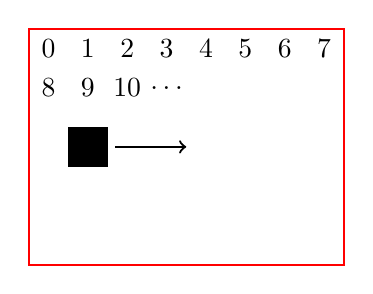
\begin{tikzpicture}
		\draw [red, thick] (0, 0) rectangle (4, -3);
		\draw [fill] (0.5, -1.25) rectangle (1, -1.75);
		\draw [->, thick] (1.1, -1.5) -- (2, -1.5);

		\foreach \i in {0, ..., 7} {
			\node at (0.5*\i + 0.25, -0.25) {\i};
		}

		\foreach \i in {0, ..., 2} {
			\pgfmathtruncatemacro{\j}{\i + 8};
			\node at (0.5*\i + 0.25, -0.75) {\j};
		}

		\node at (1.75, -0.75) {$\ldots$};
	\end{tikzpicture}
	\caption{The red box is the viewing frame of the video capture device. The black square moves under the viewing frame from left to right.}
	\label{fig:warm-up-4-experiment}
\end{figure}

\textbf{Problem:} Focus on the pixel at (0, 0). What single value represents its value over all of time? Now focus on a pixel in the same row as the black box. What single value represents its value over all time? (\textit{Hint:} don't over think it or think about actually calculating the average). Now suppose you vectorize the 2D viewing window -- count across the pixels in the frame as shown in Fig. \ref{fig:warm-up-4-experiment} and place them in a row vector in that order. Suppose there are $N$ total pixels in the frame, then the row vector should be $1 \times N$. This vector represents the values of all the pixels at one moment in time. Now create another such row vector for the next moment in time, and so on, until you have $T$ $1 \times N$ vectors. Arrange these vectors in a matrix so that each row of the matrix is one of the row vectors, and as you go down the rows of the matrix, you are advancing in time. Note that each \textit{column} of this matrix is the values of a single pixel across all values of time. What would this matrix look like for the experiment in Fig. \ref{fig:warm-up-4-experiment}? You can now choose a \textit{column} vector to represent all the columns of this matrix. What vector do you choose?